\documentclass[a4paper,11pt]{article}

% General LaTeX stuff
\usepackage{geometry} % More reasonable margins
\usepackage[utf8]{inputenc} % utf8 input good for non-ascii characters
\usepackage[T1]{fontenc} % Good for hyphenating non-ascii characters
\usepackage{lmodern}
\usepackage[british]{babel}
\usepackage{graphicx}
\usepackage[pdfusetitle]{hyperref}

% Packages for nicer appearance
\usepackage{microtype} % Improves typesetting
\usepackage[format=hang]{caption} % Format captions
\usepackage{xfrac} % Nice small fractions
% Ensure all figures are centred by default
\makeatletter
\g@addto@macro\@floatboxreset\centering
\makeatother

% Better maths support
\usepackage[intlimits]{amsmath} % intlimits option places integration limits above and below the integration sign
\usepackage{amssymb} % More maths symbols, e.g. \lesssim
\usepackage{bm} % More bold maths symbols
\usepackage{bbm} % More blackboard bold characters, via \mathbbm. Mostly for blackboard bold 1
\numberwithin{equation}{section} % Reset equation numbers in each section
\allowdisplaybreaks % Allow long maths to be broken over multiple pages

% References and citations
\usepackage{cite} % Combine multiple citations in range
\usepackage[capitalise]{cleveref} % Add automatic reference type text via \cref command
\creflabelformat{equation}{\textup{#2#1#3}} % Removes bracket around equation numbers when referencing

% Better tables
\usepackage{booktabs} % Better tables
\usepackage{array} % Allows us to define custom column types for tables
\newcolumntype{L}{>{$}l<{$}} % A left aligned maths column type

% Physics packages
\usepackage[italic]{hepnames} % Add particle name macros (e.g. \PBs)
% Remove superscript 0 from various meson macros
\renewcommand{\PBs}{\HepParticle{\PB}{\Pqs}{}\xspace}
\renewcommand{\APBs}{\HepAntiParticle{\PB}{\Pqs}{}\xspace}
\renewcommand{\PBd}{\HepParticle{\PB}{\Pqd}{}\xspace}
\usepackage{braket} % Adds Dirac bra-ket notation
\usepackage{slashed} % Adds Dirac slash notation
\usepackage{siunitx} % Add support for units
\sisetup{
	separate-uncertainty, % uncertainties with +- symbol,
	range-phrase = --, % ranges with dash
	range-units = single % only write unit once
}
\DeclareSIUnit\fb{\femto\barn}
\DeclareSIUnit\invps{\ps^{-1}}
\usepackage{suffix} % Allows us to define a starred command, for CKM macro later

% General maths macros
% Redefine Re and Im macros
\renewcommand{\Re}{\operatorname{Re}}
\renewcommand{\Im}{\operatorname{Im}}
\newcommand{\dfk}{\frac{d^4 k}{(2\pi)^4}}
\newcommand{\ddk}{\frac{d^d k}{(2\pi)^d}}
\newcommand{\dfx}{\mathop{d^4 x}}
\newcommand{\BigO}[1]{\ensuremath{\mathcal{O}\left(#1\right)}}

% General HEP macros
\newcommand{\Hamiltonian}{\ensuremath{\mathcal{H}}\xspace}
\newcommand{\Lagrangian}{\ensuremath{\mathcal{L}}\xspace}
\newcommand{\hc}{\text{h.c.}}
\newcommand{\Nc}{\ensuremath{N_c}\xspace}

% Flavour macros
\newcommand{\DeltaM}{\Delta M}
\newcommand{\DeltaG}{\Delta \Gamma}
\newcommand{\asl}{a_\text{sl}}
% Define macros for CKM elements -- the empty superscript on non-starred ensures the subscripts on starred and unstarred are level.
\newcommand{\V}[1]{\ensuremath{V_{#1}^{}}}
\WithSuffix\newcommand\V*[1]{\ensuremath{V_{#1}^*}}

\author{Matthew Kirk}
\title{Calculating polarized scattering}

\begin{document}
\maketitle



In the Dirac representation, the Gamma matrices have the following form:
\begin{align}
\gamma^0 &= \begin{pmatrix}
 1 & 0 & 0 & 0 \\
 0 & 1 & 0 & 0 \\
 0 & 0 & -1 & 0 \\
 0 & 0 & 0 & -1 \\
\end{pmatrix}
\\
\gamma^1 &= \begin{pmatrix}
 0 & 0 & 0 & 0 \\
 0 & 0 & 1 & 0 \\
 0 & -1 & 0 & 0 \\
 -1 & 0 & 0 & 0 \\
\end{pmatrix}
\\
\gamma^2 &= \begin{pmatrix}
 0 & 0 & 0 & -i \\
 0 & 0 & i & 0 \\
 0 & i & 0 & 0 \\
 -i & 0 & 0 & 0 \\
\end{pmatrix}
\\
\gamma^3 &= \begin{pmatrix}
 0 & 0 & 1 & 0 \\
 0 & 0 & 0 & -1 \\
 -1 & 0 & 0 & 0 \\
 0 & 1 & 0 & 0 \\
\end{pmatrix}
\end{align}
and the Dirac spinors look like:
% \begin{align}
% u_1 &= \sqrt{E+m} \begin{pmatrix} \cos{(\theta/2)} \\ e^{i \phi} \sin{(\theta/2)} \\ \frac{|\overrightarrow{p}|}{E+m} \cos{(\theta/2)} \\ \frac{|\overrightarrow{p}|}{E+m} e^{i \phi} \sin{(\theta/2)} \end{pmatrix}
% \\
% u_2 &= \sqrt{E+m} \begin{pmatrix} -\sin{(\theta/2)} \\ e^{i \phi} \cos{(\theta/2)} \\ \frac{|\overrightarrow{p}|}{E+m} \sin{(\theta/2)} \\ -\frac{|\overrightarrow{p}|}{E+m} e^{i \phi} \cos{(\theta/2)} \end{pmatrix}
% \\
% v_3 &= \sqrt{E+m} \begin{pmatrix} \frac{|\overrightarrow{p}|}{E+m} \sin{(\theta/2)} \\ -\frac{|\overrightarrow{p}|}{E+m} e^{i \phi} \cos{(\theta/2)} \\ -\sin{(\theta/2)} \\ e^{i \phi} \cos{(\theta/2)} \end{pmatrix}
% \\
% v_4 &= \sqrt{E+m} \begin{pmatrix}  \frac{|\overrightarrow{p}|}{E+m} \cos{(\theta/2)} \\ \frac{|\overrightarrow{p}|}{E+m} e^{i \phi} \sin{(\theta/2)} \\ \cos{(\theta/2)} \\ e^{i \phi} \sin{(\theta/2)} \end{pmatrix}
% \end{align}
\begin{align}
u_+(E, \overrightarrow{p}) &= \sqrt{E+m} \begin{pmatrix} \cos{(\theta/2)} \\  \sin{(\theta/2)} \\ \frac{|\overrightarrow{p}|}{E+m} \cos{(\theta/2)} \\ \frac{|\overrightarrow{p}|}{E+m}  \sin{(\theta/2)} \end{pmatrix}
\\
u_-(E, \overrightarrow{p}) &= \sqrt{E+m} \begin{pmatrix} -\sin{(\theta/2)} \\  \cos{(\theta/2)} \\ \frac{|\overrightarrow{p}|}{E+m} \sin{(\theta/2)} \\ -\frac{|\overrightarrow{p}|}{E+m}  \cos{(\theta/2)} \end{pmatrix}
\\
v_+(E, \overrightarrow{p}) &= \sqrt{E+m} \begin{pmatrix} \frac{|\overrightarrow{p}|}{E+m} \sin{(\theta/2)} \\ -\frac{|\overrightarrow{p}|}{E+m}  \cos{(\theta/2)} \\ -\sin{(\theta/2)} \\  \cos{(\theta/2)} \end{pmatrix}
\\
v_-(E, \overrightarrow{p}) &= \sqrt{E+m} \begin{pmatrix}  \frac{|\overrightarrow{p}|}{E+m} \cos{(\theta/2)} \\ \frac{|\overrightarrow{p}|}{E+m}  \sin{(\theta/2)} \\ \cos{(\theta/2)} \\  \sin{(\theta/2)} \end{pmatrix}
\end{align}
where $E^2 = |\overrightarrow{p}|^2 + m^2$, and $\overrightarrow{p} = (p_x, p_y, p_z) = (|\overrightarrow{p}| \sin \theta, 0, |\overrightarrow{p}| \cos \theta)$


\textbf{Bonus exercise 1:} Show that $(u_+ u_+^\dagger + u_- u_-^\dagger) \gamma^0 = \left( E \gamma^0  - \sum_{i=1}^{3} p_i \gamma^i + m \mathbbm{1}_{4x4} \right)$

\textbf{Bonus exercise 2:} Show that $(v_+ v_+^\dagger + v_- v_-^\dagger) \gamma^0 = \left( E \gamma^0  - \sum_{i=1}^{3} p_i \gamma^i - m \mathbbm{1}_{4x4} \right)$

\begin{figure}
\begin{center}
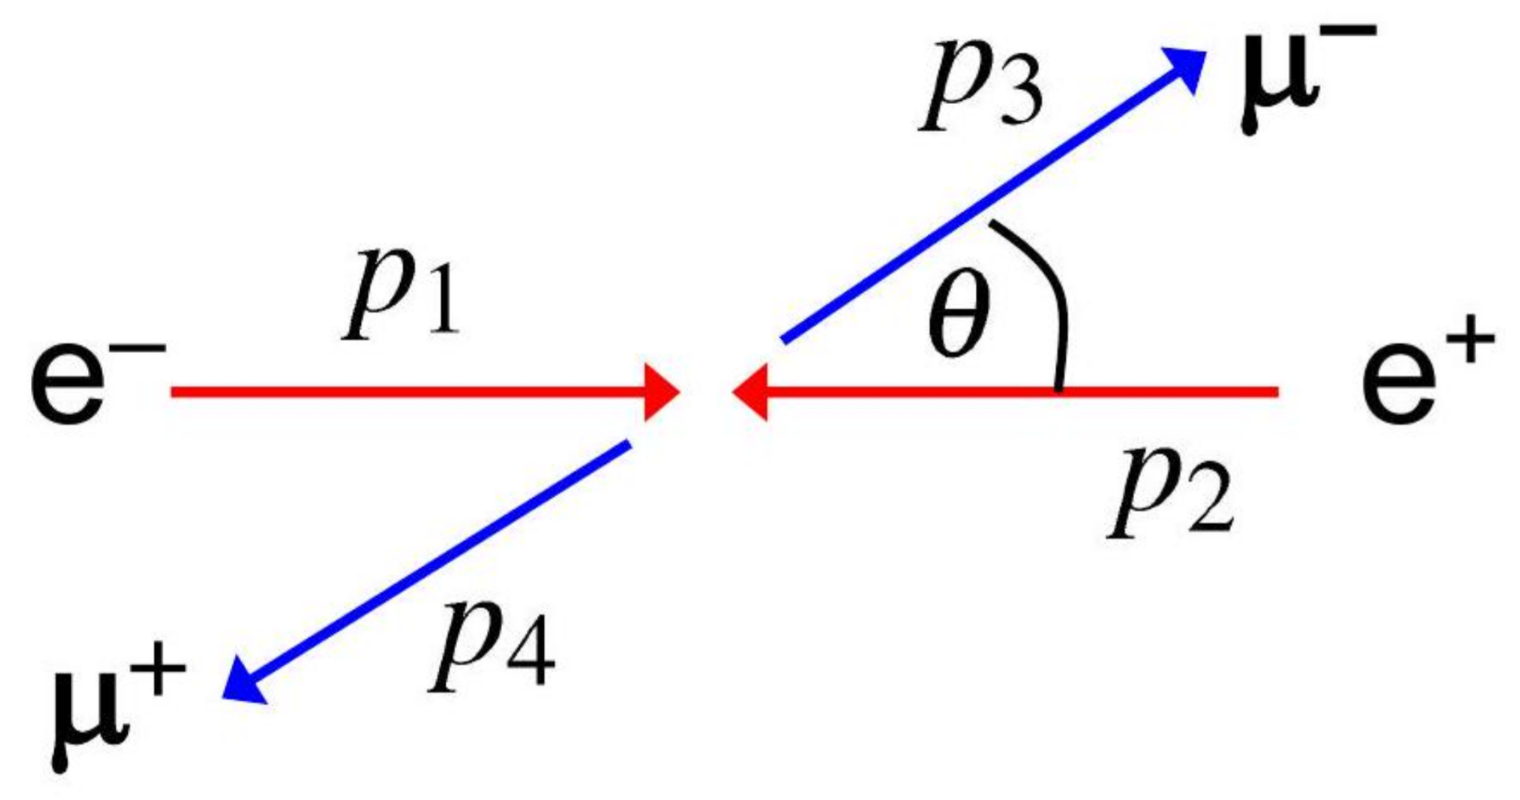
\includegraphics[width=0.7\textwidth]{scattering.png}
\end{center}
\caption{A much simpler version of the diagram you need for Exercise 1 -- talk to us for all the details}
\end{figure}



\textbf{Exercise 1:} Write down the amplitude $\mathcal{M}$ for $e^- e^+ \to \mu^- \mu^+$, assuming the initial electron and final muon both have ``$+$'' spin, and the initial positron and final state muon have ``$-$'' spin, just in terms of spinors and the gamma matrices.

\textbf{Exercise 2:} Using the representation of the spinors and gamma matrices given above, work out an explicit result for the amplitude $\mathcal{M}$.

\textbf{Exercise 3:} Using your previous answer, work out the differential cross-section
\begin{equation}
\frac{d \sigma}{d (\cos \theta)} = \frac{1}{32 \pi s} |\mathcal{M}|^2
\end{equation}
where $s = 4 E^2$.

\end{document}